\chapter{Introduction}\label{chpt:into}

\section{Graphs}
In 1736 the city of Kaliningrad, Russia was known as K\"{o}nigsberg and was part of the now defunct Kingdom of Prussia. K\"{o}nigsberg lay on either side of the Pregel river. The only way to cross the river was by a series of seven bridges. The bridges connected two large islands and are arranged as in figure \ref{fig:bridges1}. 
\begin{figure}[h]
    \centering
    
\includegraphics[height=40mm]{images/161-fig26}  %todo add image
    \caption{The bridges of K\"{o}nigsberg}
    \label{fig:bridges1}
\end{figure}
The \textit{Bridges of K\"{o}nigsberg Problem} involves finding a way to travel around the city in a way that crosses each bridge exactly once. This problem attracted the attention of Leonhard Euler. Euler noticed that the path through the land masses didn't matter. So to simplify the problem we can replace each land mass with a single point (called a vertex) and draw a line (called an edge) between two landmasses if they are connected by a bridge. We now have the representation in figure \ref{fig:bridges2}, we call this representation a graph.
\begin{figure} [h]
    \centering
        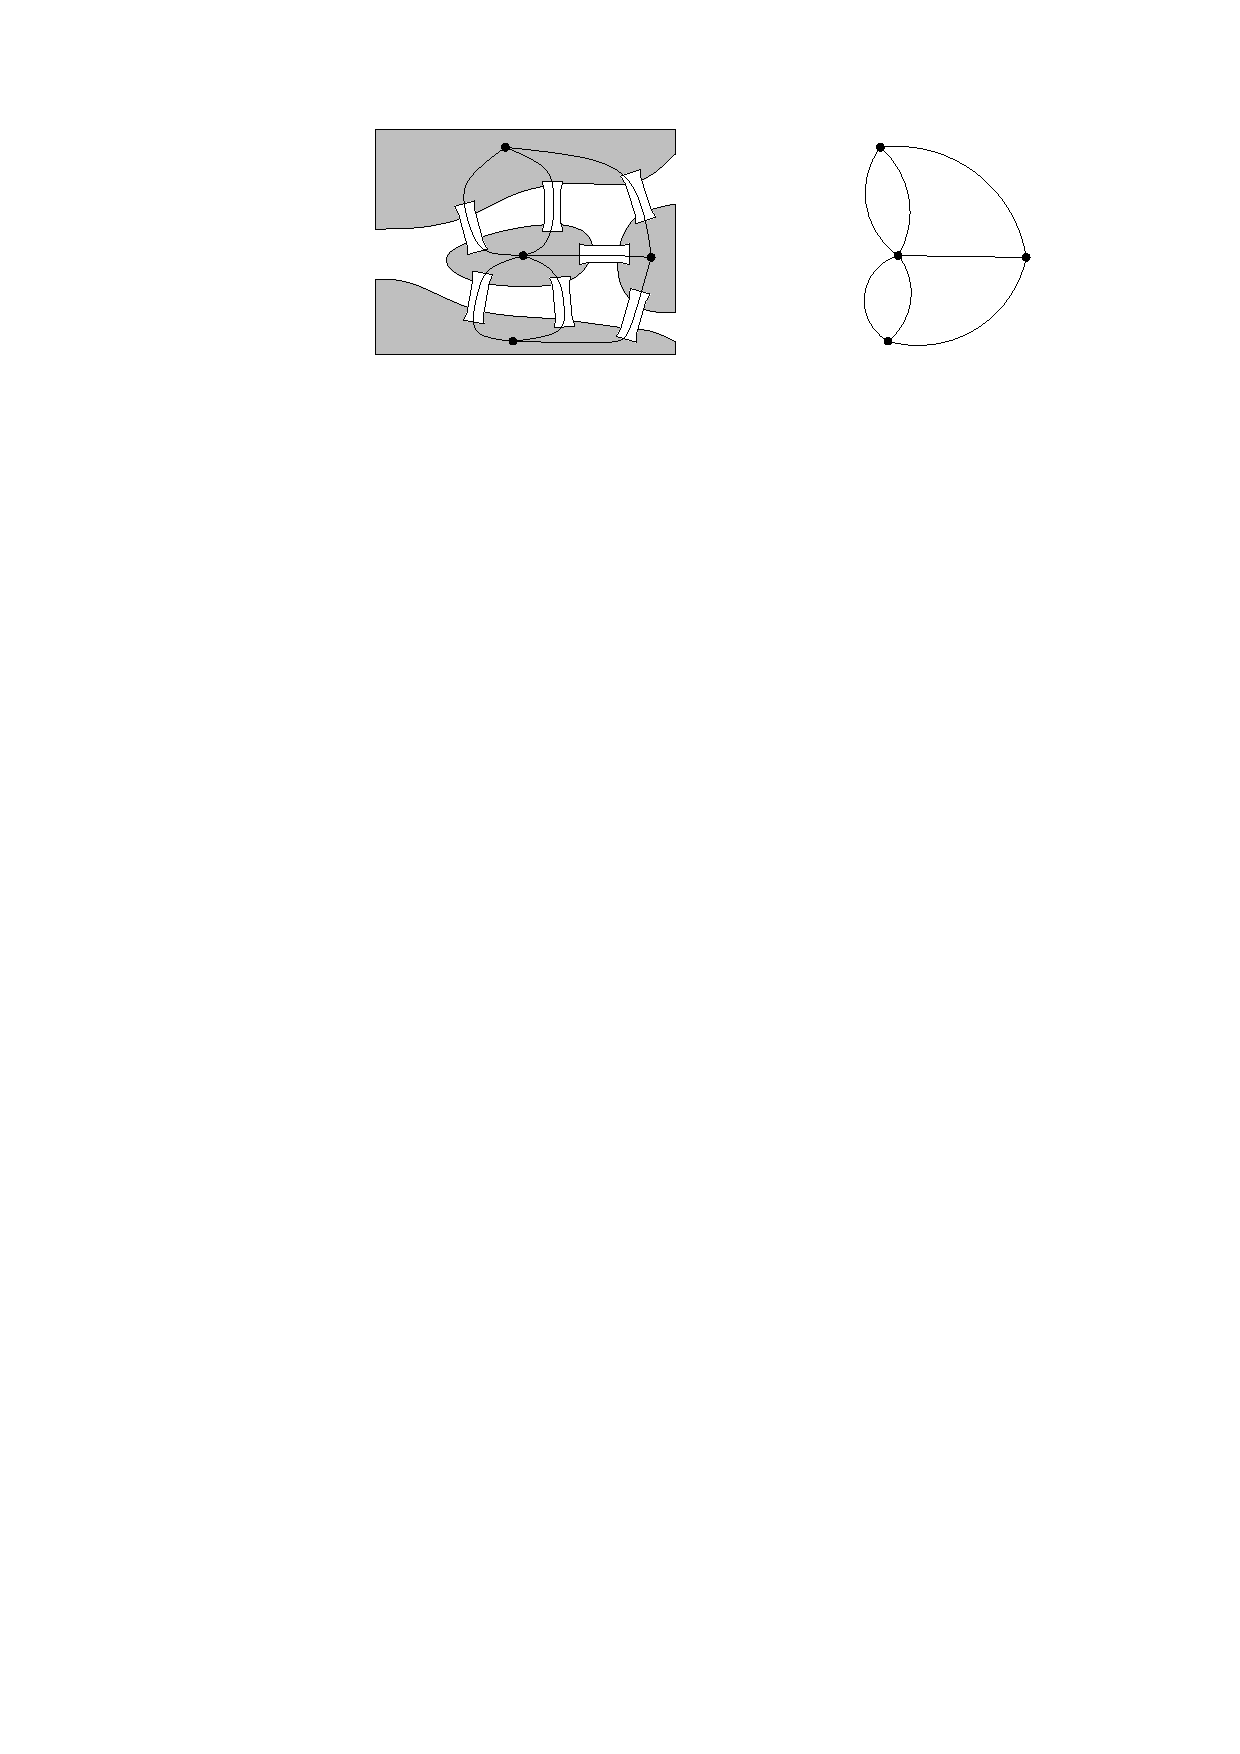
\includegraphics[height=40mm]{images/161-fig27}
    \caption{The bridges of K\"{o}nigsberg simplified}
    \label{fig:bridges2}
\end{figure} 
The problem now is to find a way to travel along each edge exactly once. Euler noticed that apart from the first and last vertex every time we enter a vertex we must also leave it. Thus the number of times we enter a vertex is the same as the number of times we leave. So, all bar two vertices must have an even number of bridges. But in our graph each vertex has an odd number of edges. This means that any path will always get stuck somewhere. Euler concludes that the bridges of K\"{o}nigsberg problem has no solution.

Euler noted that many problems can be similarly simplified. By doing this we have a way of abstracting a whole host of problems. Along with a more general notion of graph. A graph $G=(V,E)$ is a pair of vertices, $V(G)$, and edges, $E(G)$. Each edge connects two edges as is represented as a pair of vertices. The set of edges forms a relation on the vertices. For example in figure \ref{fig:k3} we have three edges $(a,b)$, $(a,c)$, and $(b,c)$. There are two main types of graphs we consider, directed graphs where the direction of the edge matters ($(a,b)\neq (b,a)$) and undirected graphs where the direction doesn't matter ($(a,b)=(b,a)$). 

\begin{figure}[h]
    \centering
\begin{tikzpicture}[scale=2]
\node[normal, label=below:$a$] (v1) at (-1.5,-1) {};
\node[normal, label=below:$b$] (v3) at (-0.5,-1) {};
\node[normal, label=below:$c$] (v2) at (-1,0) {};  
\draw (v1) edge (v2);
\draw  (v2) edge (v3);
\draw  (v3) edge (v1);
\end{tikzpicture}
    \caption{An undirected graph with three vertices and three edges}
\label{fig:k3}
\end{figure}
   
%ubiqity of graphs 
Graphs can be used to represent relationships between objects. They do this in a way that is easy to visualise and analyse. An example from recent events is COVID--19, and more generally infectious diseases.  Suppose we are in charge of monitoring an outbreak in a small country. We have a list of all the people who have contracted COVID-19. To represent the problem we consider a graph. We consider people as vertices in the graph and there to be an edge between two people if the disease could spread between them.
Then by colouring infected vertices we can easily visualise things like, who is the most infectious (who has the most infected neighbours), and where is community transmission occurring (a group of infections that are disconnected from the rest of the infections).
  
\section{Graph Algorithms}
%graph algorithms   
A graph algorithm is a set of instructions that define some procedure on a graph. An algorithm can be as simple as finding a vertex of even degree. Or more complicated, as when colouring all the vertices using only a finite number of colours.  

Suppose we are charged with laying fibre optic cable in a neighbourhood. Our goal is to use the least amount of cable possible while still connecting all the houses. We can use a graph to model the relationship between houses. The houses form the vertices and there is edge between two vertices if and only if it is possible to lay cable between the corresponding houses.
It costs different amounts to lay cable between different houses. This is because some houses are further apart, have water between them, have harder soil, etc. 
We associate each edge with a number representing the cost of laying cable between the two corresponding houses. This forms what is known as a \textit{weighted graph}. We now have all the information need to lay cable. The first step is to lay cable between the corresponding houses at the edge with the lowest cost. Next we lay cable between the corresponding houses at the edge with the least cost such that laying cable at this edge will not introduce a cycle (a closed path) of cable. By repeating this last step eventually we will have laid cable that connects all the houses. Further the cable we laid will have the least possible cost. These steps are an example of a graph algorithm. This particular algorithm is called \textit{Kruskal's algorithm}. 
 
 \section{Graph Games}  
We introduce the idea of a graph game by considering two related problems, the \textit{Dinner Party Problem} and the \textit{Dinner Party Game Problem}.

Suppose Alice is hosting a party and all the guests are mingling happily. However, the guests are hungry and need to be fed. But, they are lazy and will not move to collect food. When serving, food platters are placed around the room at the guests. A guest will take some food if a platter is placed within arm's reach. Alice needs to place platters in such a way that every guest can reach a platter. The food is expensive. So, Alice wants to place the smallest number of platters possible. The dinner party problem is, what is the minimum number of platters that Alice needs to feed everybody? 

%To see this, we can define a graph, $G$, with guests as vertices and an edge between two guests if when either of them are given a platter they will pass food between them. Minimising the number platters is now a matter of finding a set of vertices, $D$ in $G$ such that every vertex in $V(G)$ is incident to some vertex in $D$.

After the success of the first party, Alice decides to host another party. To alleviate the pressure of hosting she decides to hire a caterer, Bob. As before the platters are placed around the room. A guest will take some food if there is a platter within arms reach. Starting with Alice and on alternating turns Alice and Bob place a single platter. This continues until all the guests can be fed. As before Alice tries to use the smallest number of platters possible. Bob on the other hand makes a profit for every platter and so will try to place as many platters as possible. Bob is being paid by Alice. So, every platter he places must feed at least one new person. If not then Alice would fire Bob. If Bob was to always place a platter such that it would feed the least number of people then the total number of platters placed would be greater than the first party. Hence, Alice requires some strategy to minimise the number of platters placed. The Dinner Party Game Problem is then, what is the smallest number of platters that Alice can guarantee will always feed everyone? 
%If we define a graph as in the first party, finding a minimum number of platters is a matter of finding an optimal strategy for Alice to hand out a minimum number of platters. 
We further explore this idea in the context of the domination game and the game domination number in Chapter \ref{chpt:domSet}.

It is easy to see how this concept could be applied to other situations. For example, in wartime a nation may be trying to destroy railroads, using the minimum number of bombs possible, but their allies are secretly colluding with the enemy. Such an ally would try to make it as costly as possible to destroy railroads. Other examples include a measure of robustness in network infrastructure, scheduling, and register allocation.  

\section{Report}

The Diner Party Problem is a specific example of trying to find a minimal dominating set. To find such a set Alice would employ some algorithm. Such an algorithm may not be efficient but would solve the Dinner Party Problem. In the Dinner Party Game Problem Bob is trying to break this algorithm. Hence, we have a hostile parter as part of our graph algorithm. The algorithm will no longer solve the problem. By including Bob we have turned the algorithm into a game and a problem that is harder to solve. 

In this report 
we will explore four different graph algorithms with hostile partners. These are,
\begin{itemize}
    \item Dominating Game (Section \ref{sec:dominating_game}): \\
        Alice and Bob take turns building a dominating set.
    \item Independent Dominating Game (Section \ref{sec:ind_dom_game}): \\
        Alice and Bob take turns building a maximal independent set    
    \item Colouring Game (Section \ref{sec:colouring_game}): \\
        Alice and Bob take turns colouring a graph.
    \item Marking Game (Section \ref{sec:marking_game}): \\
        Alice and Bob take turns ordering the vertices of a graph.
\end{itemize}

In chapter \ref{chpt:domSet} we will explore the dominating and the independent dominating games. To begin we  will formally define the dominating game. We will then introduce upper and lower bounds for some classes of graphs. To bound these classes we will provide some explicit strategies for Alice. We will then extend the game to allow Alice and Bob to play more than once per turn. Finally, we will consider some bounds in the independent dominating game.

In chapter \ref{chpt:colouring} we will explore the colouring and marking games. We will begin with the standard colouring game. This game will then be extended to a version where Alice and Bob play more than once per turn. We will provide lower bounds for the colouring game. The marking game will then be introduced as a way to bound the colouring game. To do this we will use the activation strategy. We will conclude with a look at the current best bound for the class of planar graphs.

%todo why is this iteresting, applications

%todo What this this report about

%todo where has this come from

%This work has many applications in computer science and operations research, including flight scheduling, bandwidth allocation and register allocation, as well as deep theoretical interest
%note this quote is plagrisum
    
All the graph we have discussed so far are undirected. A directed graph is a graph in which each edge is assigned a direction. In such a graph the edges are no longer symmetric. That is, the edge $(a,b)$ is not the same as the edge $(b,a)$. An undirected graph can be turned into a directing graph by assigning each edge a direction. For example, in figure \ref{fig:directed_graph} we directed the graph from figure \ref{fig:k3}. %A graph that is formed this way is called an oriented graph.
%todo picture
\begin{figure}[h]
    \centering
    \begin{tikzpicture}[scale=1.5]
    \node[normal, label=below:$a$] (v1) at (-1.5,-1) {};
    \node[normal, label=below:$b$] (v3) at (-0.5,-1) {};
    \node[normal, label=below:$c$] (v2) at (-1,0) {};  
    \draw[->-=.5] (v1) to (v2);
    \draw[->-=.5]  (v2) to (v3);
    \draw[->-=.5]  (v1) to (v3);
    \end{tikzpicture}
    \caption{Directed graph}
    \label{fig:directed_graph}
\end{figure}
   
Finally, we introduce some game terminology. In a game whenever Alice or Bob has their turn by choosing a vertex we say they \textit{play} a vertex. For example, in the colouring game a play is when Alice chooses a vertex and assigns it a colour. A \textit{round} is a play of both Alice and Bob.  At any stage in the game we can consider the current dominating set along with the graph we are playing on. This pair forms a snapshot of the game detailing all the pertinent information. The size of $D$ tells you whose turn it is (Alice's if even and Bob's if odd). This snapshot is called a \textit{game state}. 

\begin{definition}[Game State]
    Let $G$ be a graph. A \textit{game state} for $G$ a sequence $\seq{v_n}$ of vertices in $V(G)$ such that each vertex appears at most once.
\end{definition}

A strategy for some game is a prescribed next move for every possible game state. In other words a strategy tells a player how to play the game. We define a strategy as a function from game states to game states. Note that the following definition only makes sense for games in which the players only pick vertices. For example in the colouring game the players assign colours to vertices. Hence the strategy would need to take this extra information into account. 

\begin{definition}[Strategy]
    For $G$ a graph and $\sigma=\seq{v_n}$ a game state for $G$ let
    \begin{align*}        
    \varphi_G &\colon {V(G)}^{<\Nn} \to {V(G)}^{<\Nn} 
    \end{align*}
    where ${V(G)}^{<\Nn}$ denotes the set of all sequences of vertices in $V(G)$. $\varphi_G$ is a strategy if it is defined on any game state and $\varphi_G(\sigma)=\sigma\caret v$ gives a legal move in the game. 
\end{definition}
    
A strategy for Alice is a strategy that is only defined on game states when it is Alice's turn. That is pairs of the form $(G,\sigma)$ where $G$ is a graph and $\sigma$ has even size. Equivalently a strategy for Bob is a strategy that is only defined on odd sized sets. 

For some fixed win condition a winning strategy for Alice is a strategy that guarantees that the game will  end with the win condition satisfied. Similarly, a winning strategy for Bob is a strategy that guarantees the game will end with the win condition being satisfied.

The formalisation of strategies provides good background to the domination game. However, to simplify proofs and intuition we will not explicitly define strategies as functions. Rather we will define the functions implicitly.    

    
    
    
    
    
    
    
    
    
    
    
    
    
    
    
    
    
    
    